% !TeX root = euclid-without-words.tex
% !TeX Program=pdfLaTeX

\documentclass[a4paper]{article}

\usepackage{verbatim}
\usepackage{tikz}
\usepackage{times}
\usepackage{bm}
\usetikzlibrary{calc, intersections, through}

\textwidth=15.5cm
\textheight=23cm
\topmargin=0pt
\headheight=0pt
\oddsidemargin=1em
\headsep=0pt
\parindent=0pt

\begin{document}
\thispagestyle{empty}

\begin{center}
\textbf{\sffamily \LARGE Euclid Without Words}

\bigskip\bigskip

\textbf{\sffamily \large Moti Ben-Ari}

\bigskip\bigskip

\textsf{\small \copyright{} CC AT-SA 2026 by Moti Ben-Ari.}
\end{center}

\vspace*{2.0cm}

%%%%%%%%%%%%%%%%%%%%%%%%%%%%%%%%%%%%%%%%%%%%%%%%%%%%%%%%%

% !TeX root = euclid-without-words.tex
% !TeX Program=pdfLaTeX
\begin{minipage}[t]{.48\textwidth}
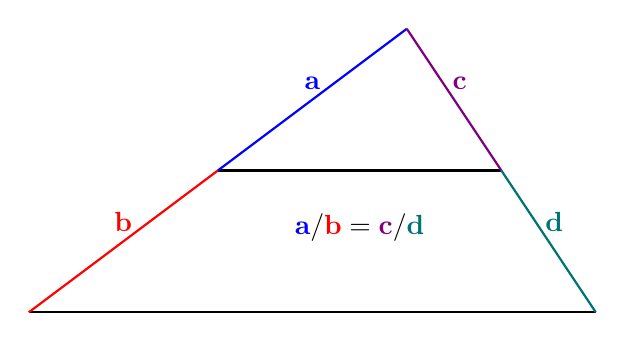
\begin{tikzpicture}[scale=1.2]

% Points of the triangle
\coordinate (a) at (0,0);
\coordinate (b) at (6,0);
\coordinate (c) at (4,3);

% Midpoints of the sides
\coordinate (mid1) at ($(a)!.5!(c)$);
\coordinate (mid2) at ($(b)!.5!(c)$);

% Base and median
\draw[thick] (a) -- (b);
\draw[thick] (mid1) -- (mid2);

% Get the median
\coordinate (midbase) at ($(a)!.5!(b)$);

% Triangle sides
\draw[thick,red] (a) -- node[above] {$\mathbf{b}$} (mid1);
\draw[thick,blue] (mid1) -- node[above] {$\mathbf{a}$} (c);
\draw[thick,black!10!teal] (b) -- 
  node[above,xshift=2pt] {$\mathbf{d}$} (mid2);
\draw[thick,violet] (mid2) -- 
  node[above,xshift=2pt] {$\mathbf{c}$} (c);

% Display formula
% Display formula
\node at ($(mid1)+(1.5,-.6)$) {$
\mathbf{\mathcolor{blue} a /
\mathcolor{red} b  = 
\mathcolor{violet} c  / 
\mathcolor{black!10!teal} d
}$};
\end{tikzpicture}
\end{minipage}

\hspace{.04\textwidth}
% !TeX root = euclid-without-words.tex
% !TeX Program=pdfLaTeX
%
% Thale's theorem 2
%
\begin{minipage}[t]{.48\textwidth}
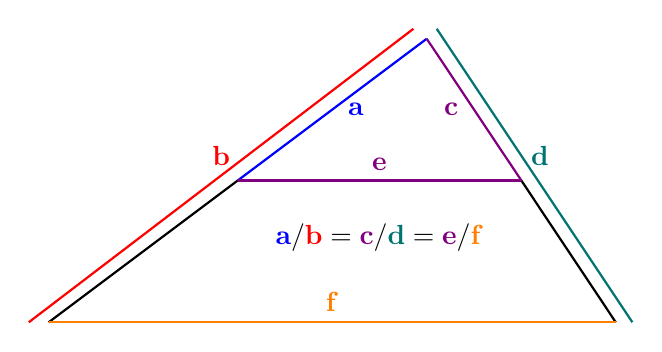
\begin{tikzpicture}[scale=1.2]
% Points of the triangle abc
\coordinate (a) at (0,0);
\coordinate (b) at (6,0);
\coordinate (c) at (4,3);

% Midpoints of the sides
\coordinate (mid1) at ($(a)!.5!(c)$);
\coordinate (mid2) at ($(b)!.5!(c)$);

% Midpoint of the base
\coordinate (midbase) at ($(a)!.5!(b)$);

% Sides of the triangle
\draw[thick] (a) -- (mid1);
\draw[thick,blue] (mid1) -- 
  node[right,xshift=2pt] {$\mathbf{a}$} (c);
\draw[thick] (b) -- (mid2);
\draw[thick,violet] (mid2) -- 
  node[left,xshift=-2pt] {$\mathbf{c}$} (c);

% Offset lines
\draw[thick,red]
  let \p1 = (a), \p2 = (c) in
    (\x1-6pt,\y1) -- node[above] {$\mathbf{b}$} (\x2-4pt,\y2+3pt);
\draw[thick,black!10!teal]
  let \p1 = (b), \p2 = (c) in
    (\x1+5pt,\y1) -- node[above,xshift=2pt] {$\mathbf{d}$} (\x2+3pt,\y2+3pt);

% Base and median
\draw[thick,orange] (a) -- node[above] {$\mathbf{f}$} (b);
\draw[thick,violet] (mid1) -- node[above] {$\mathbf{e}$} (mid2);

% Formula in color
\node at ($(mid1)+(1.5,-.6)$) {$
\mathbf{\mathcolor{blue} a /
\mathcolor{red} b  = 
\mathcolor{violet} c  / 
\mathcolor{black!10!teal} d =
\mathcolor{violet} e /
\mathcolor{orange} f
}$};
\end{tikzpicture}
\end{minipage}

\vspace*{1.0cm}

%%%%%%%%%%%%%%%%%%%%%%%%%%%%%%%%%%%%%%%%%%%%%%%%%%%%%%%%%

% !TeX root = euclid-without-words.tex
% !TeX Program=pdfLaTeX
%
% Bisector of sides is equal to one half the base
%
\begin{minipage}[t]{.48\textwidth}
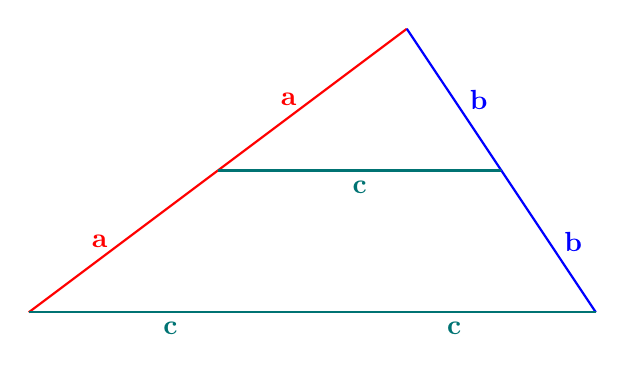
\begin{tikzpicture}[scale=1.2]

% Points of the triangle
\coordinate (a) at (0,0);
\coordinate (b) at (6,0);
\coordinate (c) at (4,3);

% Midpoints of the sides
\coordinate (mid1) at ($(a)!.5!(c)$);
\coordinate (mid2) at ($(b)!.5!(c)$);

% Midpoint of the base
\coordinate (midbase) at ($(a)!.5!(b)$);

% Draw the sides of the triangle: the base is drawn in two parts
\draw[thick,red] (a) -- node[left,xshift=-2pt] {$\mathbf{a}$} (mid1);
\draw[thick,red] (mid1) -- node[left,xshift=-2pt] {$\mathbf{a}$} (c);
\draw[thick,blue] (b) -- node[right,xshift=2pt] {$\mathbf{b}$} (mid2);
\draw[thick,blue] (mid2) -- node[right,xshift=2pt] {$\mathbf{b}$} (c);

% Draw the median
\draw[thick,black!10!teal] (mid1) -- node[below] {$\mathbf{c}$} (mid2);

% Draw the base
\draw[thick,black!10!teal] (a) -- node[below] {$\mathbf{c}$} (midbase);
\draw[thick,black!10!teal] (b) -- node[below] {$\mathbf{c}$} (midbase);
\end{tikzpicture}
\end{minipage}

\hspace{.04\textwidth}
% !TeX root = euclid-without-words.tex
% !TeX Program=pdfLaTeX
%
% Interior angle bisector
%
\begin{minipage}[t]{.48\textwidth}
\begin{tikzpicture}[baseline=-4mm,scale=1.4]

% Draw base and path two lines at known angles
\path[name path=ab] (0,0) coordinate (a) -- (0:6) coordinate (b);
\path[name path=ac] (a) -- 
  node[left,xshift=-2pt,blue] {$\mathbf{a}$} +(50:3.4);
\path[name path=bc] (b) -- 
  node[right,xshift=4pt,red] {$\mathbf{b}$} +(150:5);

% Get their intersection and draw lines to third vertex
\path[name intersections={of=ac and bc,by=c}];
\draw[blue,thick] (a) -- (c);
\draw[red,thick] (c) -- (b);

% Path bisectors of two lines
\path[name path=bisector] (c) -- +(-80:2.5);

% Intersection of angle bisector
\path [name intersections={of=bisector and ab,by=int}];

% Draw base of triangle
\draw[thick,violet] (a) -- node[below] {$\mathbf{c}$} (int);
\draw[thick,black!10!teal] (int) -- node[below] {$\mathbf{d}$} (b);

% Draw bisector and label angle
\draw[thick] (c) -- (int);
\node[below,xshift=-4pt,yshift=-10pt] at (c) {$\bm{\alpha}$};
\node[below,xshift=12pt,yshift=-10pt] at (c) {$\bm{\alpha}$};

% Display formula
\node at ($(mid1)+(1.5,-.6)$) {$
\mathbf{\mathcolor{blue} a /
\mathcolor{red} b  = 
\mathcolor{violet} c  / 
\mathcolor{black!10!teal} d
}$};
\end{tikzpicture}
\end{minipage}

\vspace*{1.0cm}

%%%%%%%%%%%%%%%%%%%%%%%%%%%%%%%%%%%%%%%%%%%%%%%%%%%%%%%%%

% !TeX root = euclid-without-words.tex
% !TeX Program=pdfLaTeX
%
% Bisector of the hypotenuse is half the hypotenuse
%
\begin{minipage}[t]{.48\textwidth}
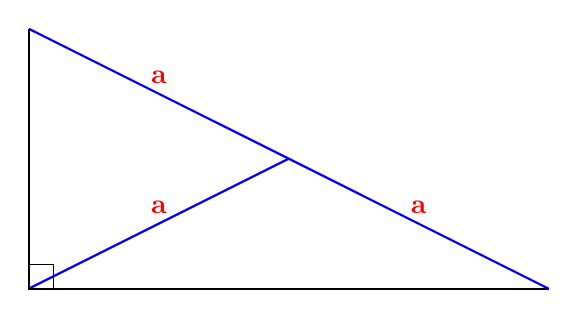
\begin{tikzpicture}[scale=1.1]
\coordinate (a) at (0,0);   % Points of the triangle
\coordinate (b) at (6,0);
\coordinate (c) at (0,3);
% Coordinate of bisector
\coordinate (hyp) at ($(b)!.5!(c)$);
% Draw the triangle and bisectors
\draw[thick] (b) -- (a) -- (c);
\draw[thick,blue] (a) -- node[above,red] {$\mathbf{a}$} (hyp);
\draw[thick,blue] (b) -- node[above,red] {$\mathbf{a}$} (hyp);
\draw[thick,blue] (c) -- node[above,red] {$\mathbf{a}$} (hyp);
% Draw square to denote right angle
\draw (a) rectangle +(8pt,8pt);
% Points at the intersections
\end{tikzpicture}
\end{minipage}

\hspace{.04\textwidth}
% !TeX root = euclid-without-words.tex
% !TeX Program=pdfLaTeX
%
% Medians of a triangle meet at a point with ratio 1:2
%
\begin{minipage}[t]{.48\textwidth}
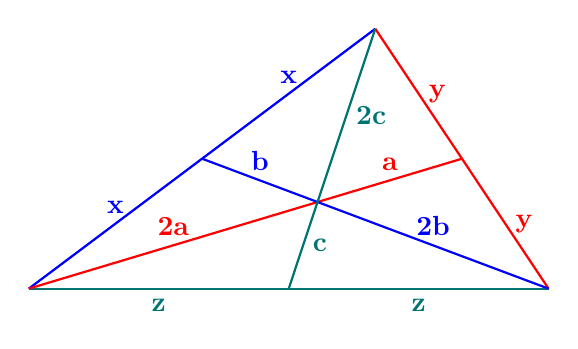
\begin{tikzpicture}[scale=1.1]
\coordinate (a) at (0,0);   % Points of the triangle
\coordinate (b) at (6,0);
\coordinate (c) at (4,3);
% Coordinates of bisectors
\coordinate (ab) at ($(a)!.5!(b)$);
\coordinate (bc) at ($(b)!.5!(c)$);
\coordinate (ac) at ($(a)!.5!(c)$);
% Draw the triangle and bisectors
\draw[blue,thick] (a) -- node[above] {$\mathbf{x}$} (ac) -- node[above] {$\mathbf{x}$} (c);
\draw[red,thick] (b) -- node[right] {$\mathbf{y}$} (bc) -- node[right] {$\mathbf{y}$} (c);
\draw[black!10!teal,thick] (a) -- node[below] {$\mathbf{z}$} (ab) -- node[below] {$\mathbf{z}$} (b);
\draw[thick,red,name path=da] (a) -- (bc);
\draw[thick,blue,name path=db] (b) -- (ac);
\draw[thick,black!10!teal,name path=dc] (c) -- (ab);
% Get their intersection
\path [name intersections={of=da and db,by={intersection}}];
% Labels
\path (a) -- node[above,red] {$\mathbf{2a}$} (intersection);
\path (bc) -- node[above,red] {$\mathbf{a}$} (intersection);
\path (b) -- node[above,blue] {$\mathbf{2b}$} (intersection);
\path (ac) -- node[above,blue] {$\mathbf{b}$} (intersection);
\path (c) -- node[right,black!10!teal] {$\mathbf{2c}$} (intersection);
\path (ab) -- node[right,black!10!teal] {$\mathbf{c}$} (intersection);
\end{tikzpicture}
\end{minipage}

\vspace*{1.0cm}

%%%%%%%%%%%%%%%%%%%%%%%%%%%%%%%%%%%%%%%%%%%%%%%%%%%%%%%%%

% !TeX root = euclid-without-words.tex
% !TeX Program=pdfLaTeX
%
% Inscribed circle center at meeting of angle bisectors
%
\begin{minipage}[t]{.48\textwidth}
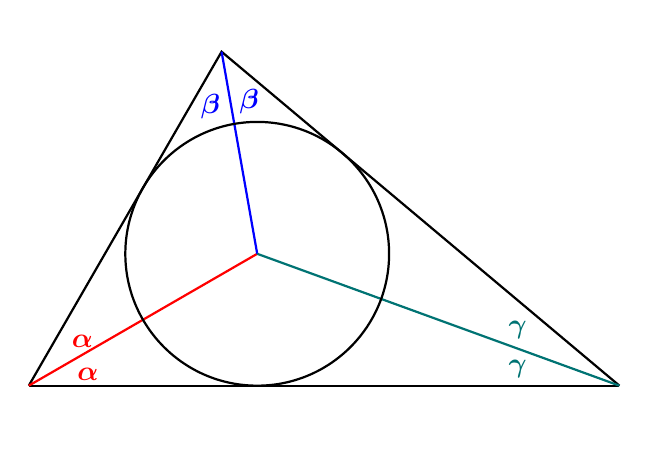
\begin{tikzpicture}[baseline=-6mm,scale=1.5]
% Draw base and path two lines at known angles
\draw[thick] (0,0) coordinate (a) -- (0:5) coordinate (b);
\path[name path=ac] (a) -- +(60:3.5);
\path[name path=bc] (b) -- +(140:4.5);
% Get their intersection and draw lines to third vertex
\path[name intersections={of=ac and bc,by=c}];
\draw[thick] (a) -- (c) -- (b);
% Path bisectors of two lines
\path[name path=bia,blue] (a) -- +(30:3.6);
\path[name path=bib,red] (b) -- +(160:5);
% Intersection of angle bisectors
\path [name intersections={of=bia and bib,by=center}];
%% Draw angle bisectors to center
\draw[thick,red] (a) -- (center);
\draw[thick,blue] (c) -- (center);
\draw[thick,black!10!teal] (b) -- (center);
%% Labels of angles
\node[red,right,xshift=14pt,yshift=4pt] at (a) {$\bm{\alpha}$};
\node[red,right,xshift=12pt,yshift=16pt] at (a) {$\bm{\alpha}$};
\node[blue,below,xshift=-4pt,yshift=-12pt] at (c) {$\bm{\beta}$};
\node[blue,below,xshift=10pt,yshift=-10pt] at (c) {$\bm{\beta}$};
\node[black!10!teal,left,xshift=-30pt,yshift=6pt] at (b) {$\bm{\gamma}$};
\node[black!10!teal,left,xshift=-30pt,yshift=20pt] at (b) {$\bm{\gamma}$};
%% Get perpendicular from center to one side and draw circle
\coordinate (perp) at ($(a)!(center)!(b)$);
\node [thick,draw,circle through=(perp)] at (center) {};
\end{tikzpicture}
\end{minipage}

\hspace{.04\textwidth}
% !TeX root = euclid-without-words.tex
% !TeX Program=pdfLaTeX
%
% Perpendicular bisectors meet in the center of the circumscribed circle
%
\begin{minipage}[t]{.48\textwidth}
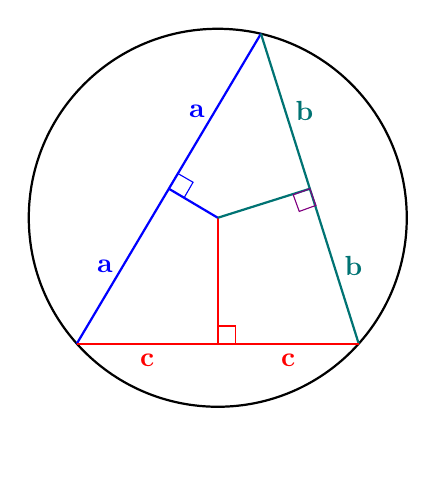
\begin{tikzpicture}[scale=.8,baseline=-30mm]
% Circle goes from (a) to (b)
\coordinate (a) at (0,0);
\coordinate (b) at (6,0);
% Line containing lower points is (c) -- (d)
\coordinate (c) at (0,-2);
\coordinate (d) at (6,-2);
% Line containing upper points is (e) -- (f)
\coordinate (e) at (0,2);
\coordinate (f) at (4,3);
% Name the two chords
\path [name path=chord1] (c) -- (d);
\path [name path=chord2] (e) -- (f);
% Name the coordinate of the center of the circle
\coordinate (center) at ($ (a)!.5!(b) $);
% Draw a circle whose center is half-way between (a) and (b) through (a)
\node [draw,thick,circle through=(a),name path=circ] at (center) {};
% Get intersections of the upper and lower lines with the circle
\path [name intersections={of=circ and chord1,by={i1,i2}}];
\path [name intersections={of=circ and chord2,by={i3,i4}}];
% Draw triangle
\draw [thick,blue] (i1) -- node[left] {$\mathbf{a}$} ($(i1)!.5!(i3)$) --
  node[left] {$\mathbf{a}$} (i3);
\draw[thick,black!10!teal] (i3) -- node[right] {$\mathbf{b}$} ($(i3)!.5!(i2)$) --
  node[right] {$\mathbf{b}$} (i2);
\draw[thick,red] (i2) -- node[below] {$\mathbf{c}$} ($(i2)!.5!(i1)$) -- 
  node[below] {$\mathbf{c}$} (i1);
% Draw three perpendicular bisectors
\draw [thick,red,fill] (center) -- ($(i1)!(center)!(i2)$);
\draw [thick,blue,fill] (center) -- ($(i1)!(center)!(i3)$);
\draw [thick,black!10!teal,fill] (center) -- ($(i2)!(center)!(i3)$);
% Draw squares to denote right angles
\draw[red] ($ (i1) !.5! (i2) $) rectangle +(8pt,8pt);
\draw[blue,rotate=-30] ($ (i1) !.5! (i3) $) rectangle +(8pt,8pt);
\draw[violet,rotate=-160] ($ (i3) !.5! (i2) $)
  rectangle +(8pt,8pt);
\end{tikzpicture}
\end{minipage}

\vspace*{1.0cm}

%%%%%%%%%%%%%%%%%%%%%%%%%%%%%%%%%%%%%%%%%%%%%%%%%%%%%%%%%

% !TeX root = euclid-without-words.tex
% !TeX Program=pdfLaTeX
%
% Inscribed angle one half of central angle
%
\begin{minipage}[t]{.48\textwidth}
\hspace{3em}
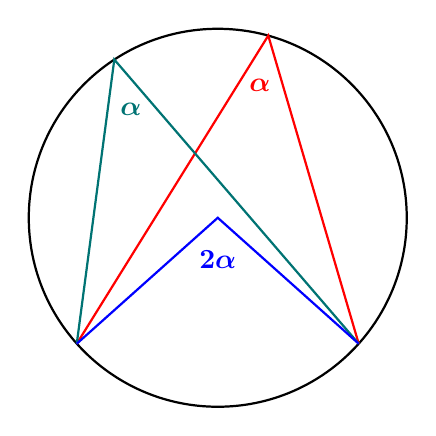
\begin{tikzpicture}[scale=.8]
% Circle goes from (a) to (b)
\coordinate (a) at (0,0);
\coordinate (b) at (6,0);
\coordinate (center) at (3,0);
% Line containing lower points is (c) -- (d)
\coordinate (c) at (0,-2);
\coordinate (d) at (6,-2);
% Line containing upper points is (e) -- (f);
\coordinate (e) at (0,2.3);
\coordinate (f) at (4.5,3);
% Name the upper and lower lines
\path [name path=chord1] (c) -- (d);
\path [name path=chord2] (e) -- (f);
% Draw a circle whose center is half-way between (a) and (b) through (a)
\node [draw,thick,circle through=(a),name path=circ] at (center) {};
% Get intersections of the upper and lower lines with the circle
\path [name intersections={of=circ and chord1,by={i1,i2}}];
\path [name intersections={of=circ and chord2,by={i3,i4}}];
% Draw the lower chord
%\draw[thick] (i1) -- (i2);
% Draw the two subtended angles and the center angle
\draw[thick,red] (i1) -- (i3)
  node[below,xshift=-3pt,yshift=-12pt] {$\bm{\alpha}$} -- (i2);
\draw[thick,black!10!teal] (i1) -- (i4)
  node[below,xshift=6pt,yshift=-12pt] {$\bm{\alpha}$} -- (i2);
\draw[thick,blue] (i1) -- (center)
  node[below,yshift=-8pt] {$\bm{2\alpha}$} -- (i2);
\end{tikzpicture}
\end{minipage}

\hspace{.04\textwidth}
% !TeX root = euclid-without-words.tex
% !TeX Program=pdfLaTeX
%
% Angles of tangent and angle subtending a chord are equal
%
\begin{minipage}[t]{.48\textwidth}
\hspace{3em}
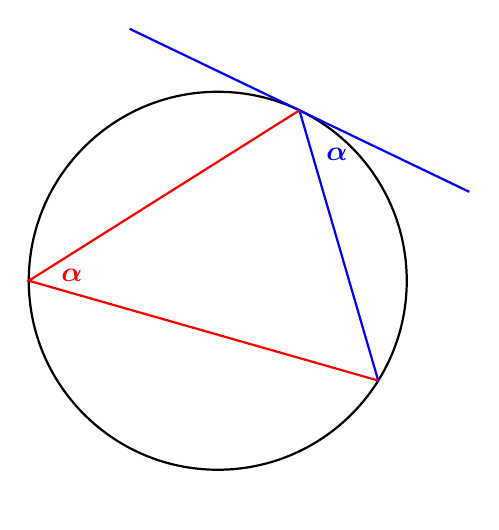
\begin{tikzpicture}[scale=.8,baseline=-80pt]
% Circle goes from (a) to (b)
\coordinate (a) at (0,0);
\coordinate (b) at (6,0);
% Line containing lower point (d)
\coordinate (d) at (7,-2);
% Point outside circle is (e)
\coordinate (e) at (1.6,4);
% Name the lower chord
\path [name path=chord] (a) -- (d);
% Draw a circle whose center is half-way between (a) and (b) through (a)
\node [draw,thick,circle through=(a),name path=circ] (circle) at ($ (a)!.5!(b) $) {};
% Get intersection of the lower line with the circle
\path [name intersections={of=circ and chord,by={i1,i2}}];
% Draw the tangent line
\coordinate (tan) at (tangent cs:node=circle, point={(e)}, solution=2);
\draw[thick,blue] (e) -- ($ (e)!2!(tan) $);
% Draw the triangle
\draw [thick,blue] (tan) node[below right,xshift=6pt,yshift=-10pt] {$\bm{\alpha}$} -- (i2);
\draw [thick,red] (tan) -- (a) node[right,xshift=8pt,yshift=2pt] {$\bm{\alpha}$} -- (i2);
\end{tikzpicture}
\end{minipage}

\vspace*{1.0cm}

%%%%%%%%%%%%%%%%%%%%%%%%%%%%%%%%%%%%%%%%%%%%%%%%%%%%%%%%%

% !TeX root = euclid-without-words.tex
% !TeX Program=pdfLaTeX
%
% Intersecting tangents
%
\begin{minipage}[t]{.48\textwidth}
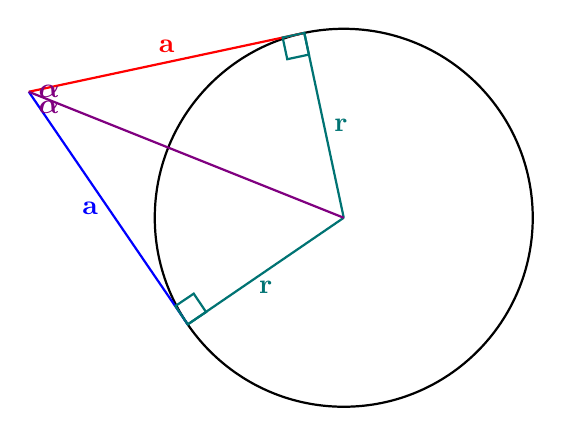
\begin{tikzpicture}[scale=.8]
% Circle goes from (a) to (b)
\coordinate (a) at (0,0);
\coordinate (b) at (6,0);
\coordinate (center) at (3,0);
% Point outside circle is (e)
\coordinate (e) at (-2,2);
\node [draw,thick,circle through=(a),name path=circ] (circle) at (center) {};
% Draw the tangent line
\coordinate (tan1) at (tangent cs:node=circle, point={(e)}, solution=1);
\coordinate (tan2) at (tangent cs:node=circle, point={(e)}, solution=2);
\draw[thick,blue] (e) -- node[left] {$\mathbf{a}$} (tan1);
\draw[thick,red] (e) -- node[above] {$\mathbf{a}$} (tan2);
% Draw radii
\draw[thick,black!10!teal] (center) -- node[below] {$\mathbf{r}$} (tan1);
\draw[thick,black!10!teal] (center) -- node[right] {$\mathbf{r}$} (tan2);
% Draw line from exterior point to center
\draw[thick,violet] (e) -- (center);
% Draw right angles
\draw[thick,black!10!teal,rotate=34] (tan1) rectangle +(10pt,10pt);
\draw[thick,black!10!teal,rotate=-168] (tan2) rectangle +(10pt,10pt);
% Label angles
\node [violet,right] at (e) {$\bm{\alpha}$};
\node [violet,below right] at (e) {$\bm{\alpha}$};
\end{tikzpicture}
\end{minipage}

\hspace{.04\textwidth}
% !TeX root = euclid-without-words.tex
% !TeX Program=pdfLaTeX
%
% Intersecting secants
%
\begin{minipage}[t]{.48\textwidth}
\hspace{4em}
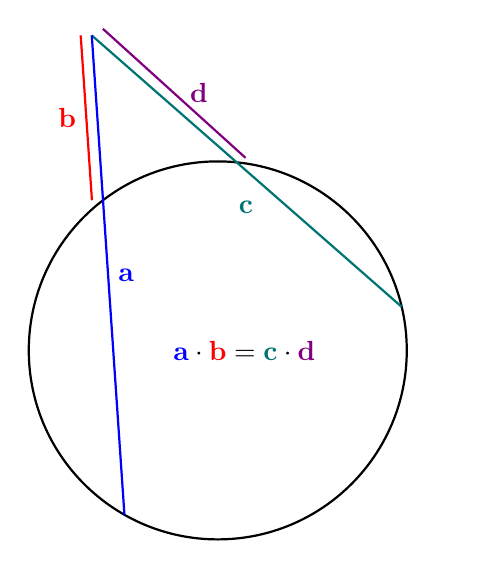
\begin{tikzpicture}[scale=.8]
% Circle goes from (a) to (b)
\coordinate (a) at (0,0);
\coordinate (b) at (6,0);
% Line containing lower points is (c) -- (d)
\coordinate (c) at (1,-3);
\coordinate (d) at (7,1.5);
% Point outside circle is (e)
\coordinate (e) at (1,5);
% Name the lower chord
\path [name path=chord] (c) -- (d);
% Draw a circle whose center is half-way between (a) and (b) through (a)
\coordinate (mid) at ($ (a)!.5!(b) $);	
\node [draw,thick,circle through=(a),name path=circ] at (mid) {};
% Get intersection of the lower line with the circle
\path [name intersections={of=circ and chord,by={i1,i2}}];
% Draw the full secants
\draw [name path=secant1,thick,black!10!teal] (i1) -- node[left,xshift=6pt,yshift=-13pt] {$\mathbf{c}$} (e);
\draw [name path=secant2,thick,blue] (i2) -- node[right] {$\mathbf{a}$} (e);
% Get intersections of the secants with the circle
\path [name intersections={of=circ and secant1,by={s11,s12}}];
\path [name intersections={of=circ and secant2,by={s21,s22}}];
% Draw offset lines from outside point with the intersections of the secants
\draw[thick,red]
  let \p1 = (s21), \p2 = (e) in
    (\x2-5pt,\y2) -- node[left] {$\mathbf{b}$} (\x1-5pt,\y1);
\draw[thick,violet]
  let \p1 = (s12), \p2 = (e) in
    (\x2+5pt,\y2+3pt) -- node[right,xshift=2pt] {$\mathbf{d}$} (\x1+4pt,\y1+2pt);
% Display formula in color
\node at ($(mid)+(12pt,0)$) {$
\mathbf{\mathcolor{blue} a \cdot
\mathcolor{red} b  = 
\mathcolor{black!10!teal} c  \cdot
\mathcolor{violet} d
}$};
\end{tikzpicture}
\end{minipage}

\vspace*{1.0cm}

%%%%%%%%%%%%%%%%%%%%%%%%%%%%%%%%%%%%%%%%%%%%%%%%%%%%%%%%%

% !TeX root = euclid-without-words.tex
% !TeX Program=pdfLaTeX
%
% Intersecting tangent and secant
%
\begin{minipage}[t]{.48\textwidth}
\hspace{4em}
\begin{tikzpicture}[scale=.8]
% Circle goes from (a) to (b)
\coordinate (a) at (0,0);
\coordinate (b) at (6,0);
% Line containing lower points is (c) -- (d)
\coordinate (c) at (1,-3);
\coordinate (d) at (7,1.5);
% Point outside circle is (e)
\coordinate (e) at (1,5);
% Name the lower chord
\path [name path=chord] (c) -- (d);
% Draw a circle whose center is half-way between (a) and (b) through (a)
\coordinate (mid) at ($ (a)!.5!(b) $);
\node [draw,thick,circle through=(a),name path=circ] at (mid) {};
% Get intersection of the lower line with the circle
\path [name intersections={of=circ and chord,by={i1,i2}}];
% Draw the full secant
\draw [name path=secant2,thick,blue] (i2) -- node[right] {$\mathbf{a}$} (e);
% Get intersection of the secant with the circle
\path [name intersections={of=circ and secant2,by={s21,s22}}];
% Draw offset line from outside point with the intersection of the secant
\draw[thick,red]
  let \p1 = (s21), \p2 = (e) in
    (\x2-5pt,\y2) -- node[left] {$\mathbf{b}$} (\x1-5pt,\y1);
% Draw the tangent line
\coordinate (tan) at (tangent cs:node=circle, point={(e)}, solution=2);
\draw[thick,black!10!teal] (e) -- node[right,yshift=4pt] {$\mathbf{c}$} (tan);
% Display formula in color
\node at ($(mid)+(12pt,0)$) {$
\mathbf{\mathcolor{black!10!teal} c^2
= 
\mathcolor{blue} a \cdot
\mathcolor{red} b
}$};
\end{tikzpicture}
\end{minipage}

\hspace{.04\textwidth}
% !TeX root = euclid-without-words.tex
% !TeX Program=pdfLaTeX
%
% Intersecting chords
%
\begin{minipage}[t]{.48\textwidth}
\hspace{4em}
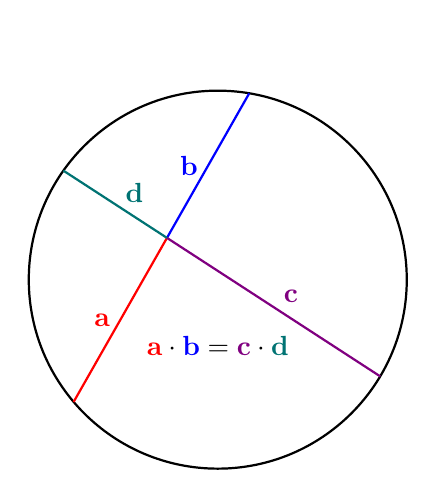
\begin{tikzpicture}[scale=.8]
% Circle goes from (a) to (b)
\coordinate (a) at (0,0);
\coordinate (b) at (6,0);
% Line containing lower points is (c) -- (d)
\coordinate (c) at (0,-2);
\coordinate (d) at (6,-1.5);
% Line containing upper points is (e) -- (f)
\coordinate (e) at (0,1.5);
\coordinate (f) at (6,4);
% Name the upper and lower lines
\path [name path=chord1] (c) -- (d);
\path [name path=chord2] (e) -- (f);
% Draw a circle whose center is half-way between (a) and (b) through (a)
\coordinate (mid) at ($ (a)!.5!(b) $);
\node [draw,thick,circle through=(a),name path=circ] at (mid) {};
% Get intersections of the upper and lower lines with the circle
\path [name intersections={of=circ and chord1,by={i1,i2}}];
\path [name intersections={of=circ and chord2,by={i3,i4}}];
% Name the two chords
\path [name path=x1] (i1) -- (i3);
\path [name path=x2] (i2) -- (i4);
% Get their intersection
\path [name intersections={of=x1 and x2,by={p}}];
% Draw four lines from intersection to circle
\draw[thick,red] (i1) -- node[left] {$\mathbf{a}$} (p);
\draw[thick,blue] (p) --  node[left] {$\mathbf{b}$} (i3);
\draw[thick,violet] (i2) -- node[right,yshift=4pt] {$\mathbf{c}$} (p);
\draw[thick,black!10!teal] (p) -- node[right,yshift=4pt] {$\mathbf{d}$} (i4);
% Display formula in color
\node at ($(mid)+(0pt,-30pt)$) 
{$
\mathbf{\mathcolor{red} a \cdot
\mathcolor{blue} b  = 
\mathcolor{violet} c  \cdot
\mathcolor{black!10!teal} d
}$};
\end{tikzpicture}
\end{minipage}

\vspace*{1.0cm}

%%%%%%%%%%%%%%%%%%%%%%%%%%%%%%%%%%%%%%%%%%%%%%%%%%%%%%%%%

% !TeX root = euclid-without-words.tex
% !TeX Program=pdfLaTeX
%
% Sums of opposite sides of circumscribed quadrilateral are equal
%
\begin{minipage}[t]{.48\textwidth}
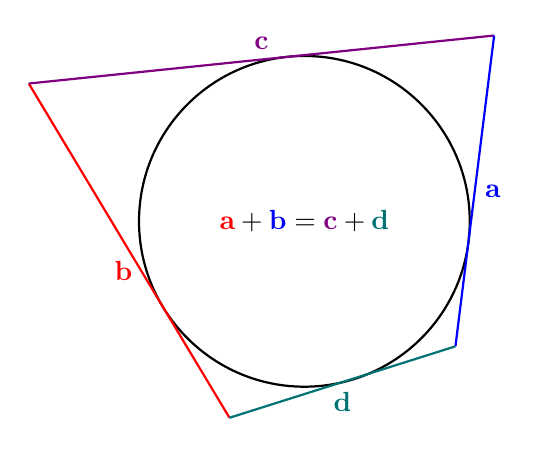
\begin{tikzpicture}[scale=.7]
% Circle goes from (a) to (b)
\coordinate (x) at (0,3);
\coordinate (y) at (6,3);
\coordinate (a) at (-2,5.5);
% Draw a circle whose center is half-way between (x) and (y) through (x)
\coordinate (mid) at ($ (x)!.5!(y) $);
\node [draw,thick,circle through=(x),name path=circ] (circle) at (mid) {};
% Draw tangent lines
\coordinate (tan1) at (tangent cs:node=circle, point={(a)}, solution=1);
\draw[thick,red] (a) -- node[below,xshift=-2pt] {$\mathbf{b}$}
  ($(a)!1.5!(tan1)$) coordinate (b);
\coordinate (tan2) at (tangent cs:node=circle, point={(a)}, solution=2);
\draw[thick,violet] (a) -- node[above] {$\mathbf{c}$}
  ($(a)!1.8!(tan2)$) coordinate (c);
\coordinate (tan3) at (tangent cs:node=circle, point={(c)}, solution=2);
\draw[thick,blue] (c) -- node[right] {$\mathbf{a}$}
  ($(c)!1.51!(tan3)$)  coordinate (d);
\draw[thick,black!10!teal] (b) -- node[below] {$\mathbf{d}$} (d);
% Display formula in color
\node at (mid) {$
\mathbf{\mathcolor{red} a +
\mathcolor{blue} b  = 
\mathcolor{violet} c  +
\mathcolor{black!10!teal} d
}$};
\end{tikzpicture}
\end{minipage}

\hspace{.04\textwidth}
% !TeX root = euclid-without-words.tex
% !TeX Program=pdfLaTeX
%
% Opposite angles in an inscribed quadrilateral add up to 180
%
\begin{minipage}[t]{.48\textwidth}
\hspace{4em}
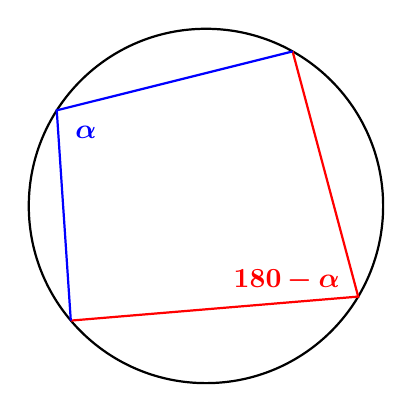
\begin{tikzpicture}[scale=.75]
% Circle goes from (a) to (b)
\coordinate (a) at (0,0);
\coordinate (b) at (6,0);
% Line containing lower points is (c) -- (d)
\coordinate (c) at (0,-2);
\coordinate (d) at (6,-1.5);
% Line containing upper points is (e) -- (f)
\coordinate (e) at (0,1.5);
\coordinate (f) at (6,3);
% Name the upper and lower lines
\path [name path=chord1] (c) -- (d);
\path [name path=chord2] (e) -- (f);
% Draw a circle whose center is half-way between (a) and (b) through (a)
\coordinate (mid) at ($ (a)!.5!(b) $);
\node [draw,thick,circle through=(a),name path=circ] (circle) at (mid) {};
%\node [draw,thick,circle through=(a),name path=circ] at ($ (a)!.5!(b) $) {};
% Get intersections of the upper and lower lines with the circle
\path [name intersections={of=circ and chord1,by={i1,i2}}];
\path [name intersections={of=circ and chord2,by={i3,i4}}];
% Draw the two subtended angles
\draw[thick,red] (i1) -- (i2)
  node[left,xshift=-3pt,yshift=6pt] {$\bm{180-\alpha}$} -- (i3);
\draw[thick,blue] (i1) -- (i4)
  node[right,xshift=3pt,yshift=-8pt] {$\bm{\alpha}$} -- (i3);
\end{tikzpicture}
\end{minipage}

\vspace*{1.0cm}

%%%%%%%%%%%%%%%%%%%%%%%%%%%%%%%%%%%%%%%%%%%%%%%%%%%%%%%%%

% !TeX root = euclid-without-words.tex
% !TeX Program=pdfLaTeX
%
% Diagonals of parallelogram bisect each other
%
\begin{minipage}[t]{.48\textwidth}
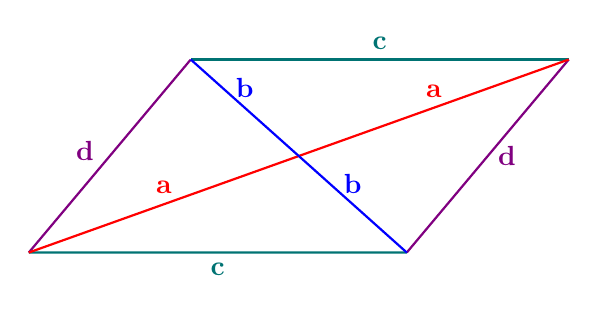
\begin{tikzpicture}[scale=.8]
% Bottom side of parallelogram
\coordinate (a) at (0,0);
\coordinate (b) at (6,0);
% Draw parallelogram at angle 50
\draw[thick,violet] (a) -- node[left,xshift=-2pt,yshift=2pt] {$\mathbf{d}$} +(50:4) coordinate (c);
\draw[thick,black!10!teal] (c) -- node[above] {$\mathbf{c}$} +(6,0) coordinate (d);
\draw[thick,violet] (d) -- node[right] {$\mathbf{d}$} +(230:4) coordinate (b);
\draw[thick,black!10!teal] (b) -- node[below] {$\mathbf{c}$} (a);
% Name the two diagonals
\path [name path=d1] (a) -- (d);
\path [name path=d2] (b) -- (c);
% Get their intersection
\path [name intersections={of=d1 and d2,by={intersection}}];
% Draw diagonals
\draw[thick,red] (a) -- node[above] {$\mathbf{a}$} (intersection);
\draw[thick,red] (intersection) -- node[above] {$\mathbf{a}$} (d);
\draw[thick,blue] (b) -- node[above] {$\mathbf{b}$} (intersection);
\draw[thick,blue] (intersection) -- node[above] {$\mathbf{b}$} (c);
\end{tikzpicture}
\end{minipage}

\hspace{.04\textwidth}
% !TeX root = euclid-without-words.tex
% !TeX Program=pdfLaTeX
%
% Diagonals of rhombus bisect each other and are perpendicular
%
\begin{minipage}[t]{.48\textwidth}
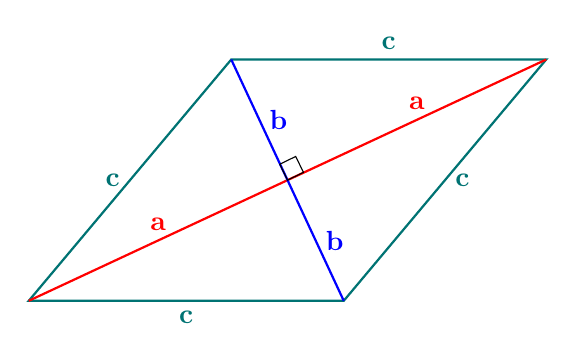
\begin{tikzpicture}[scale=.8]
% Bottom side of rhombus
\coordinate (a) at (0,0);
\coordinate (b) at (5,0);
% Draw rhombus at angle 50
\draw[thick,black!10!teal] (a) -- 
  node[left] {$\mathbf{c}$} ++(50:5) coordinate (c) -- 
  node[above] {$\mathbf{c}$} ++(5,0) coordinate (d) -- 
  node[right] {$\mathbf{c}$} (b) -- node[below] {$\mathbf{c}$} cycle;
% Name the two diagonals
\path [name path=d1] (a) -- (d);
\path [name path=d2] (b) -- (c);
% Get their intersection
\path [name intersections={of=d1 and d2,by={intersection}}];
% Draw diagonals
\draw[thick,red] (a) -- node[above] {$\mathbf{a}$} (intersection);
\draw[thick,red] (intersection) -- node[above] {$\mathbf{a}$} (d);
\draw[thick,blue] (b) -- node[right] {$\mathbf{b}$} (intersection);
\draw[thick,blue] (intersection) -- node[right] {$\mathbf{b}$} (c);
% Draw square to denote right angle
\draw[rotate=26] (intersection) rectangle +(8pt,8pt);
\end{tikzpicture}
\end{minipage}

\vspace*{1.0cm}

%%%%%%%%%%%%%%%%%%%%%%%%%%%%%%%%%%%%%%%%%%%%%%%%%%%%%%%%%

% !TeX root = euclid-without-words.tex
% !TeX Program=pdfLaTeX
%
% Diagonals of a kite
%
\begin{minipage}[t]{.48\textwidth}
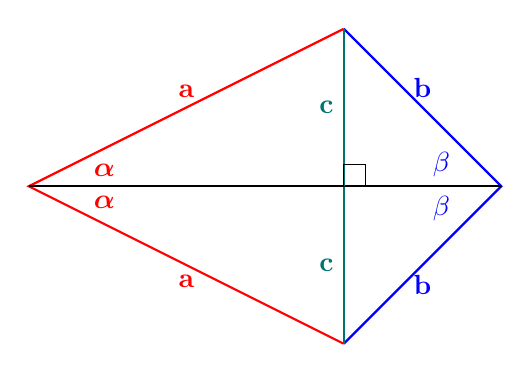
\begin{tikzpicture}[scale=1]
% Draw the kite
\coordinate (a) at (0,0);
\coordinate (b) at (4,2);
\coordinate (c) at (6,0);
\coordinate (d) at (4,-2);
\coordinate (intersection) at (4,0);
\draw[red,thick] (d) -- node[below] {$\mathbf{a}$} (a) -- node[above] {$\mathbf{a}$} (b);
\draw[blue,thick] (b) -- node[above] {$\mathbf{b}$} (c) -- node[below] {$\mathbf{b}$} (d);
% Label nodes
\node[red,above right,xshift=20pt] at (a) {$\bm{\alpha}$};
\node[red,below right,xshift=20pt] at (a) {$\bm{\alpha}$};
\node[blue,above left,xshift=-15pt] at (c) {$\mathbf{\beta}$};
\node[blue,below left,xshift=-15pt] at (c) {$\mathbf{\beta}$};
% Draw diagonals
\draw[thick] (a) -- (c);
\draw[black!10!teal,thick] (b) -- node[left] {$\mathbf{c}$}(intersection) -- node[left] {$\mathbf{c}$} (d);

% Draw square to denote right angle
\draw (intersection) rectangle +(8pt,8pt);
\end{tikzpicture}
\end{minipage}

\hspace{.04\textwidth}
% !TeX root = euclid-without-words.tex
% !TeX Program=pdfLaTeX
%
% Median of a trapezoid is average of sides
%
\begin{minipage}[t]{.48\textwidth}
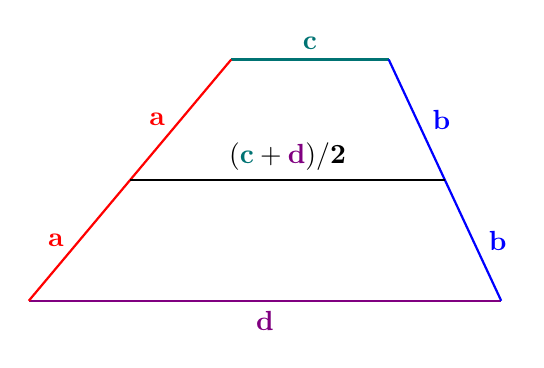
\begin{tikzpicture}
% Bottom of trapeze
\coordinate (a) at (0,0);
\coordinate (b) at (6,0);
% Draw the bases of the trapeze
\draw[thick,violet] (a) -- node[below] {$\mathbf{d}$} (b);
\path (a) -- ++(50:4) coordinate (c) -- ++(2,0) coordinate (d);
\draw[thick,black!10!teal] (c) -- node[above] {$\mathbf{c}$} (d);
% Draw the sides of the trapeze in two parts
\coordinate (mid1) at ($(a)!.5!(c)$);
\coordinate (mid2) at ($(b)!.5!(d)$);
\draw[thick,red] (a) -- node[left,xshift=-2pt] {$\mathbf{a}$} (mid1);
\draw[thick,red] (mid1) -- node[left,xshift=-2pt] {$\mathbf{a}$} (c);
\draw[thick,blue] (b) -- node[right,xshift=2pt] {$\mathbf{b}$} (mid2);
\draw[thick,blue] (mid2) -- node[right,xshift=2pt] {$\mathbf{b}$} (d);
% Draw the median
\draw[thick] (mid1) -- (mid2);

% Formula in color
\coordinate (center) at ($(mid1)!.5!(mid2)$);
\node at ($(center)+(0,.3)$) {$
\mathbf{
(\mathcolor{black!10!teal} c +
\mathcolor{violet} d ) / 2
}$};
\end{tikzpicture}
\end{minipage}

\vspace*{1.0cm}

%%%%%%%%%%%%%%%%%%%%%%%%%%%%%%%%%%%%%%%%%%%%%%%%%%%%%%%%%

% !TeX root = euclid-without-words.tex
% !TeX Program=pdfLaTeX
\begin{minipage}[t]{.48\textwidth}
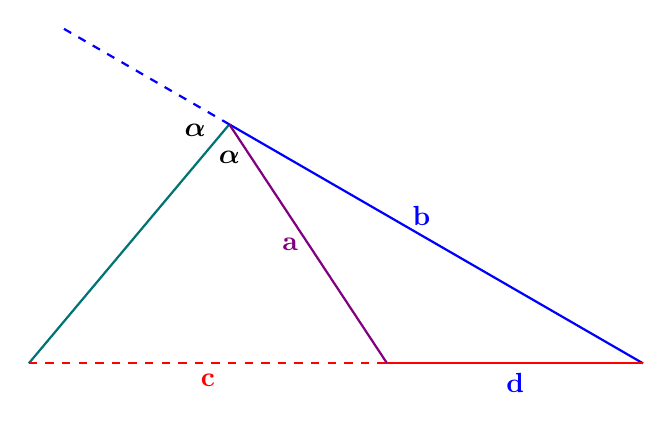
\begin{tikzpicture}[scale=1.3]
% Draw base and path two lines at known angles
\path[name path=ab] (0,0) coordinate (a) -- (6,0) coordinate (b);
\path[name path=ac] (a) -- +(50:3.4);
\path[name path=bc] (b) -- node[above,blue] {$\mathbf{b}$} +(150:5);
% Get their intersection and draw lines to third vertex
\path[name intersections={of=ac and bc, by=c}];
\draw[blue,thick] (c) -- (b);
\draw[black!10!teal,thick] (a) -- (c);
% Extend lines
\draw[blue,thick,dashed] (c) -- ($(b)!1.4!(c)$);
\coordinate (d) at (3.5,0);
\draw[violet, thick] (d) -- node[left,violet] {$\mathbf{a}$} (c);
\draw[thick,red,dashed] (a) -- node[red,below] {$\mathbf{c}$} (d);
\draw[thick,red] (d) -- node[blue,below] {$\mathbf{d}$} (b);
% Label angles
\node[below,xshift=0pt,yshift=-6pt] at (c) {$\bm{\alpha}$};
\node[left,xshift=-5pt,yshift=-2pt] at (c) {$\bm{\alpha}$};
\end{tikzpicture}
(\end{minipage}

\hspace{.04\textwidth}
% !TeX root = euclid-without-words.tex
% !TeX Program=pdfLaTeX
%
% Altitudes meet in the orthocenter
%
\begin{minipage}[t]{.48\textwidth}
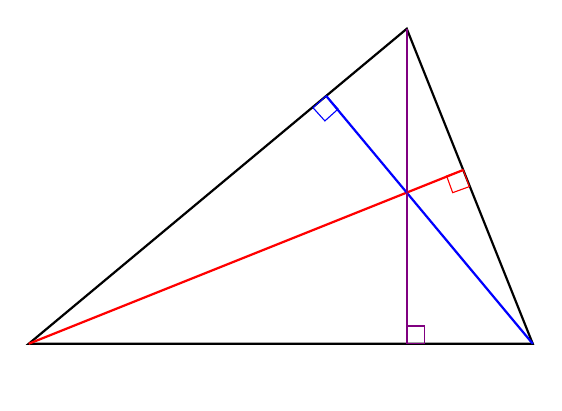
\begin{tikzpicture}[scale=.8,baseline=-5mm]
% Triangle
\coordinate (a) at (0,0);
\coordinate (b) at (8,0);
\coordinate (c) at (6,5);
\draw[thick] (a) -- (b) -- (c) -- cycle;
% Draw altitudes
\draw[thick,red] (a) -- ($(b)!(a)!(c)$) coordinate (pa);
\draw[thick,blue] (b) -- ($(a)!(b)!(c)$) coordinate (pb);
\draw[thick,violet] (c) -- ($(a)!(c)!(b)$) coordinate (pc);
% Draw right angle squares
\draw[red,rotate=-160] (pa) rectangle +(8pt,8pt);
\draw[blue,rotate=-138] (pb) rectangle +(8pt,8pt);
\draw[violet] (pc) rectangle +(8pt,8pt);
\end{tikzpicture}
\end{minipage}

\vspace*{1.0cm}

%%%%%%%%%%%%%%%%%%%%%%%%%%%%%%%%%%%%%%%%%%%%%%%%%%%%%%%%%

% !TeX root = euclid-without-words.tex
% !TeX Program=pdfLaTeX

% Euler line and nine-point circle

\begin{minipage}[t]{.48\textwidth}
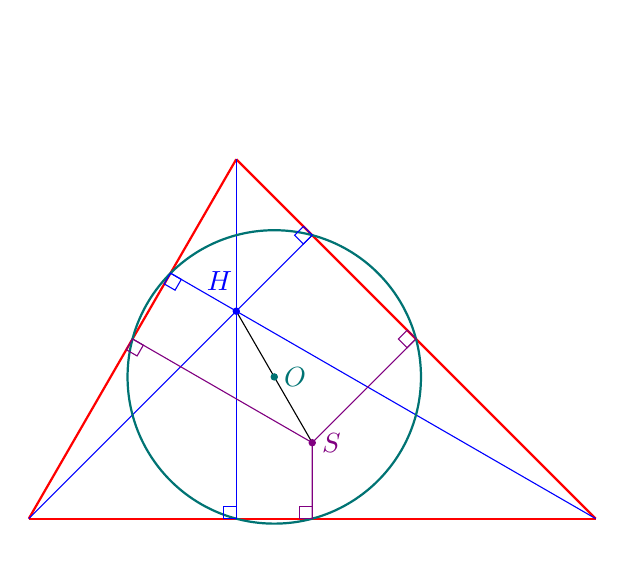
\begin{tikzpicture}[scale=.9,baseline=-5mm]
\def\A{60}
\def\B{135}

% Triangle
\coordinate (A) at (0,0);
\coordinate (B) at (8,0);
\path[name path=ac] (A) -- +(\A:8);
\path[name path=bc] (B) -- +(\B:9);
\path [name intersections = {of = ac and bc, by = {C} }];
\draw[name path=ab,red,thick] (A) -- (B);
\draw[red,thick] (B) -- (C);
\draw[red,thick] (C) -- (A);

% Altitudes
\draw[name path=calt,blue] (C) -- ($(A)!(C)!(B)$) coordinate (D);
\draw[name path=aalt,blue] (A) -- ($(B)!(A)!(C)$) coordinate (E);
\draw[name path=balt,blue] (B) -- ($(A)!(B)!(C)$) coordinate (FF);
\path [name intersections = {of = aalt and calt, by = {H} }];

% Perpendicular bisectors
\coordinate (G) at ($(A)!.5!(B)$);
\coordinate (F) at ($(A)!.5!(C)$);
\coordinate (GG) at ($(B)!.5!(C)$);
\path[name path=abperp] (F) -- +(\A-90:5);
\path[name path=acperp] (G) -- +(90:6);
\path [name intersections = {of = abperp and acperp, by = {S} }];
\draw[violet] (F) -- (S) -- (G);
\draw[violet] (S) -- (GG);

% Draw Euler line and nine-point circle
\draw (S) -- (H);
\coordinate (O) at ($(H)!.5!(S)$);
\node[draw,circle through=(F),black!10!teal,thick] at (O) {};

% Label nodes
\fill[black!10!teal] (O) circle (1.5pt);
\fill[violet] (S) circle (1.5pt);
\fill[blue] (H) circle (1.5pt);
\node[blue,above left,,xshift=2pt,yshift=4pt] at (H) {$H$};
\node[right,black!10!teal] at (O) {$O$};
\node[right,violet] at (S) {$S$};

% Right angles
\draw[rotate=90,blue] (D) rectangle +(5pt,5pt);
\draw[rotate=135,blue] (E) rectangle +(5pt,5pt);
\draw[rotate=-120,blue] (FF) rectangle +(5pt,5pt);
\draw[rotate=-120,violet] (F) rectangle +(5pt,5pt);
\draw[rotate=135,violet] (GG) rectangle +(5pt,5pt);
\draw[rotate=90,violet] (G) rectangle +(5pt,5pt);
\end{tikzpicture}
\end{minipage}

\hspace{.04\textwidth}
% !TeX root = euclid-without-words.tex
% !TeX Program=pdfLaTeX
%
% Median of a trapezoid is average of sides
%
\begin{minipage}[t]{.48\textwidth}
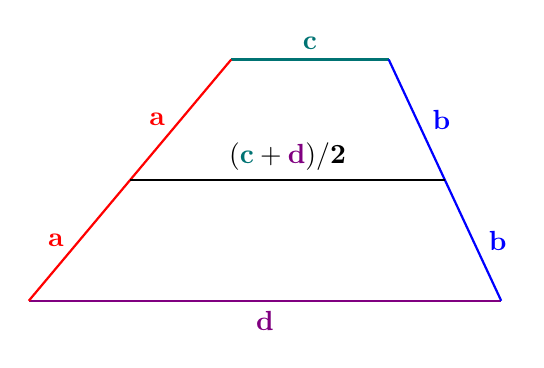
\begin{tikzpicture}
% Bottom of trapeze
\coordinate (a) at (0,0);
\coordinate (b) at (6,0);
% Draw the bases of the trapeze
\draw[thick,violet] (a) -- node[below] {$\mathbf{d}$} (b);
\path (a) -- ++(50:4) coordinate (c) -- ++(2,0) coordinate (d);
\draw[thick,black!10!teal] (c) -- node[above] {$\mathbf{c}$} (d);
% Draw the sides of the trapeze in two parts
\coordinate (mid1) at ($(a)!.5!(c)$);
\coordinate (mid2) at ($(b)!.5!(d)$);
\draw[thick,red] (a) -- node[left,xshift=-2pt] {$\mathbf{a}$} (mid1);
\draw[thick,red] (mid1) -- node[left,xshift=-2pt] {$\mathbf{a}$} (c);
\draw[thick,blue] (b) -- node[right,xshift=2pt] {$\mathbf{b}$} (mid2);
\draw[thick,blue] (mid2) -- node[right,xshift=2pt] {$\mathbf{b}$} (d);
% Draw the median
\draw[thick] (mid1) -- (mid2);

% Formula in color
\coordinate (center) at ($(mid1)!.5!(mid2)$);
\node at ($(center)+(0,.3)$) {$
\mathbf{
(\mathcolor{black!10!teal} c +
\mathcolor{violet} d ) / 2
}$};
\end{tikzpicture}
\end{minipage}

\vspace*{1.0cm}

%%%%%%%%%%%%%%%%%%%%%%%%%%%%%%%%%%%%%%%%%%%%%%%%%%%%%%%%%

% !TeX root = euclid-without-words.tex
% !TeX Program=pdfLaTeX
%
% Chord angles
%
\begin{minipage}[t]{.48\textwidth}
\hspace{4em}
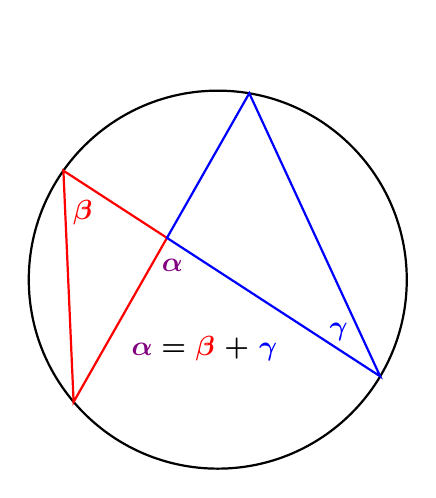
\begin{tikzpicture}[scale=.8]
% Circle goes from (a) to (b)
\coordinate (a) at (0,0);
\coordinate (b) at (6,0);
% Line containing lower points is (c) -- (d)
\coordinate (c) at (0,-2);
\coordinate (d) at (6,-1.5);
% Line containing upper points is (e) -- (f)
\coordinate (e) at (0,1.5);
\coordinate (f) at (6,4);
% Name the upper and lower lines
\path [name path=chord1] (c) -- (d);
\path [name path=chord2] (e) -- (f);
% Draw a circle whose center is half-way between (a) and (b) through (a)
\coordinate (mid) at ($ (a)!.5!(b) $);
\node [draw,thick,circle through=(a),name path=circ] at (mid) {};
% Get intersections of the upper and lower lines with the circle
\path [name intersections={of=circ and chord1,by={i1,i2}}];
\path [name intersections={of=circ and chord2,by={i3,i4}}];
% Name the two chords
\path [name path=x1] (i1) -- (i3);
\path [name path=x2] (i2) -- (i4);
% Get their intersection
\path [name intersections={of=x1 and x2,by={p}}];
% Draw four lines from intersection to circle
\draw[thick,red] (i1) -- (p) -- 
  (i4) node[red,below,xshift=7pt,yshift=-7pt] {$\bm{\beta}$} -- cycle;
\draw[thick,blue] (i2) node[blue,above,xshift=-15pt,yshift=9pt] {$\bm{\gamma}$} -- (p) -- (i3) -- cycle;
\node[thick,violet,below,xshift=2pt,yshift=-4pt] at (p) {$\bm{\alpha}$};
% Display formula in color
\begin{scope}[xshift=1.8cm,yshift=-1.2cm]
\node[anchor=base,violet] at (0,0) {$\bm{\alpha}$};
\node[anchor=base] at (.5,0) {$\bm{=}$};
\node[anchor=base,red] at (1.0,0) {$\bm{\beta}$};
\node[anchor=base] at (1.5,0) {$\bm{+}$};
\node[anchor=base,blue] at (2,0) {$\bm{\gamma}$};
\end{scope}
\end{tikzpicture}
\end{minipage}

\hspace{.04\textwidth}
% !TeX root = euclid-without-words.tex
% !TeX Program=pdfLaTeX
%
% Secant chord
%
\begin{minipage}[t]{.48\textwidth}
%\hspace{4em}
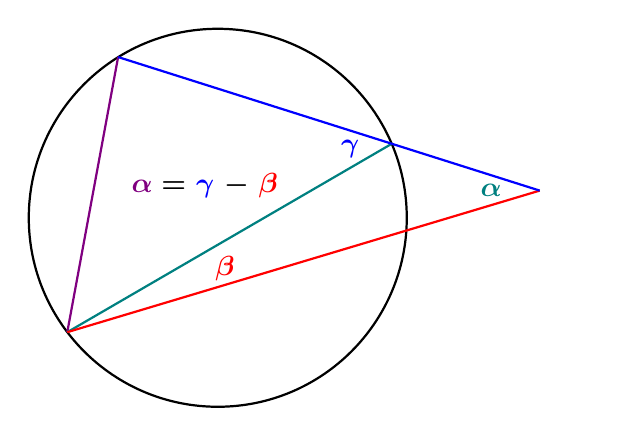
\begin{tikzpicture}[scale=.8]
% Circle goes from (a) to (b)
\coordinate (a) at (0,0);
\coordinate (b) at (6,0);
% Line containing lower points is (c) -- (d)
\coordinate (c) at (0,-2);
\coordinate (d) at (6,-.2);
% Line containing upper points is (e) -- (f)
\coordinate (e) at (0,3);
\coordinate (f) at (6,1.1);
% Name the upper and lower lines
\path [name path=chord1] (c) -- (d);
\path [name path=chord2] (e) -- (f);
% Draw a circle whose center is half-way between (a) and (b) through (a)
\coordinate (mid) at ($ (a)!.5!(b) $);
\node [draw,thick,circle through=(a),name path=circ] at (mid) {};
% Get intersections of the upper and lower lines with the circle
\path [name intersections={of=circ and chord1,by={i1,i2}}];
\path [name intersections={of=circ and chord2,by={i3,i4}}];
% Name the two chords
\path [name path=x1] (i1) -- (i3);
\path [name path=x2] (i2) -- (i4);
\draw[thick,violet] (i1) -- (i4);
\draw[thick,teal] (i1) -- (i3) 
  node[left,blue,xshift=-8pt,yshift=-2pt] {$\bm{\gamma}$};
\path[name path=x1] (i1) 
  node[above right,red,xshift=50pt,yshift=15pt] {$\bm{\beta}$} -- 
  ($(i1)!1.5!(i2)$);
\path[name path=x2] (i4) -- ($(i4)!1.8!(i3)$);
% Get their intersection
\path [name intersections={of=x1 and x2,by={p}}];
\draw[thick,red] (i1) -- (p) node[left,teal,xshift=-10pt] {$\bm{\alpha}$};
\draw[thick,blue] (i4) -- (p);
% Display formula in color
\begin{scope}[xshift=1.8cm,yshift=.4cm]
\node[anchor=base,violet] at (0,0) {$\bm{\alpha}$};
\node[anchor=base] at (.5,0) {$\bm{=}$};
\node[anchor=base,blue] at (1.0,0) {$\bm{\gamma}$};
\node[anchor=base] at (1.5,0) {$\bm{-}$};
\node[anchor=base,red] at (2,0) {$\bm{\beta}$};
\end{scope}
\end{tikzpicture}
\end{minipage}

\vspace*{1.0cm}


\end{document}
